\documentclass[border=10pt]{standalone}
\usepackage{pgfplots}
\pgfplotsset{compat=1.18}
\begin{document}
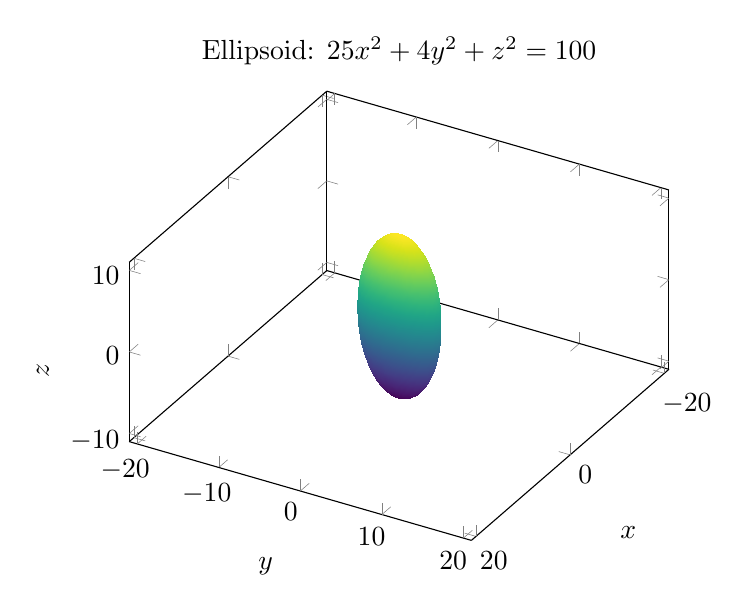
\begin{tikzpicture}
\begin{axis}[
    view={120}{30},
    xlabel=$x$, ylabel=$y$, zlabel=$z$,
    xmin=-3, xmax=3,
    ymin=-6, ymax=6,
    zmin=-11, zmax=11,
    axis equal,
    title={Ellipsoid: $25x^2+4y^2+z^2=100$},
    colormap/viridis
]
\addplot3[
    surf,
    shader=interp,
    samples=40,
    samples y=60,
    domain=0:180,
    y domain=0:360,
    z buffer=sort
]
({2*sin(x)*cos(y)}, {5*sin(x)*sin(y)}, {10*cos(x)});
\end{axis}
\end{tikzpicture}
\end{document}
